\chapter{Резюме на глава 5: Работни процеси}
\label{chapter-case-study}

В тази глава обсъждаме два автоматизирани работни процеса за обмен на данни за биологичното разнообразие, разработени като част от OpenBiodiv: (1) автоматично внасяне на записи за наблюдения на видове (occurrence data) в ръкописи и (2) автоматично генериране на ръкописни материали от екологичните метаданни (EML). Работните потоци бяха представени на webinar за организацията iDigBio и публикувани като научна статия (\cite{senderov_online_2016}).

Слайдовете от презентацията под \url{https://github.com/vsenderov/idigbio-webinar}.

\section{Резултати и дискусия}

\subsection{Работен процес 1: Автоматизиран импорт на occurrence data в ръкописи, разработени в ARPHA Writing Tool}

Разработихме автоматичент импорт на occurrence data в таксономична статия в системата ARPHA от международните бази данни GBIF, BOLD, iDigBio и PlutoF (Фиг.:\ref{Workflow-idigbio}).

\begin{figure}
\centering
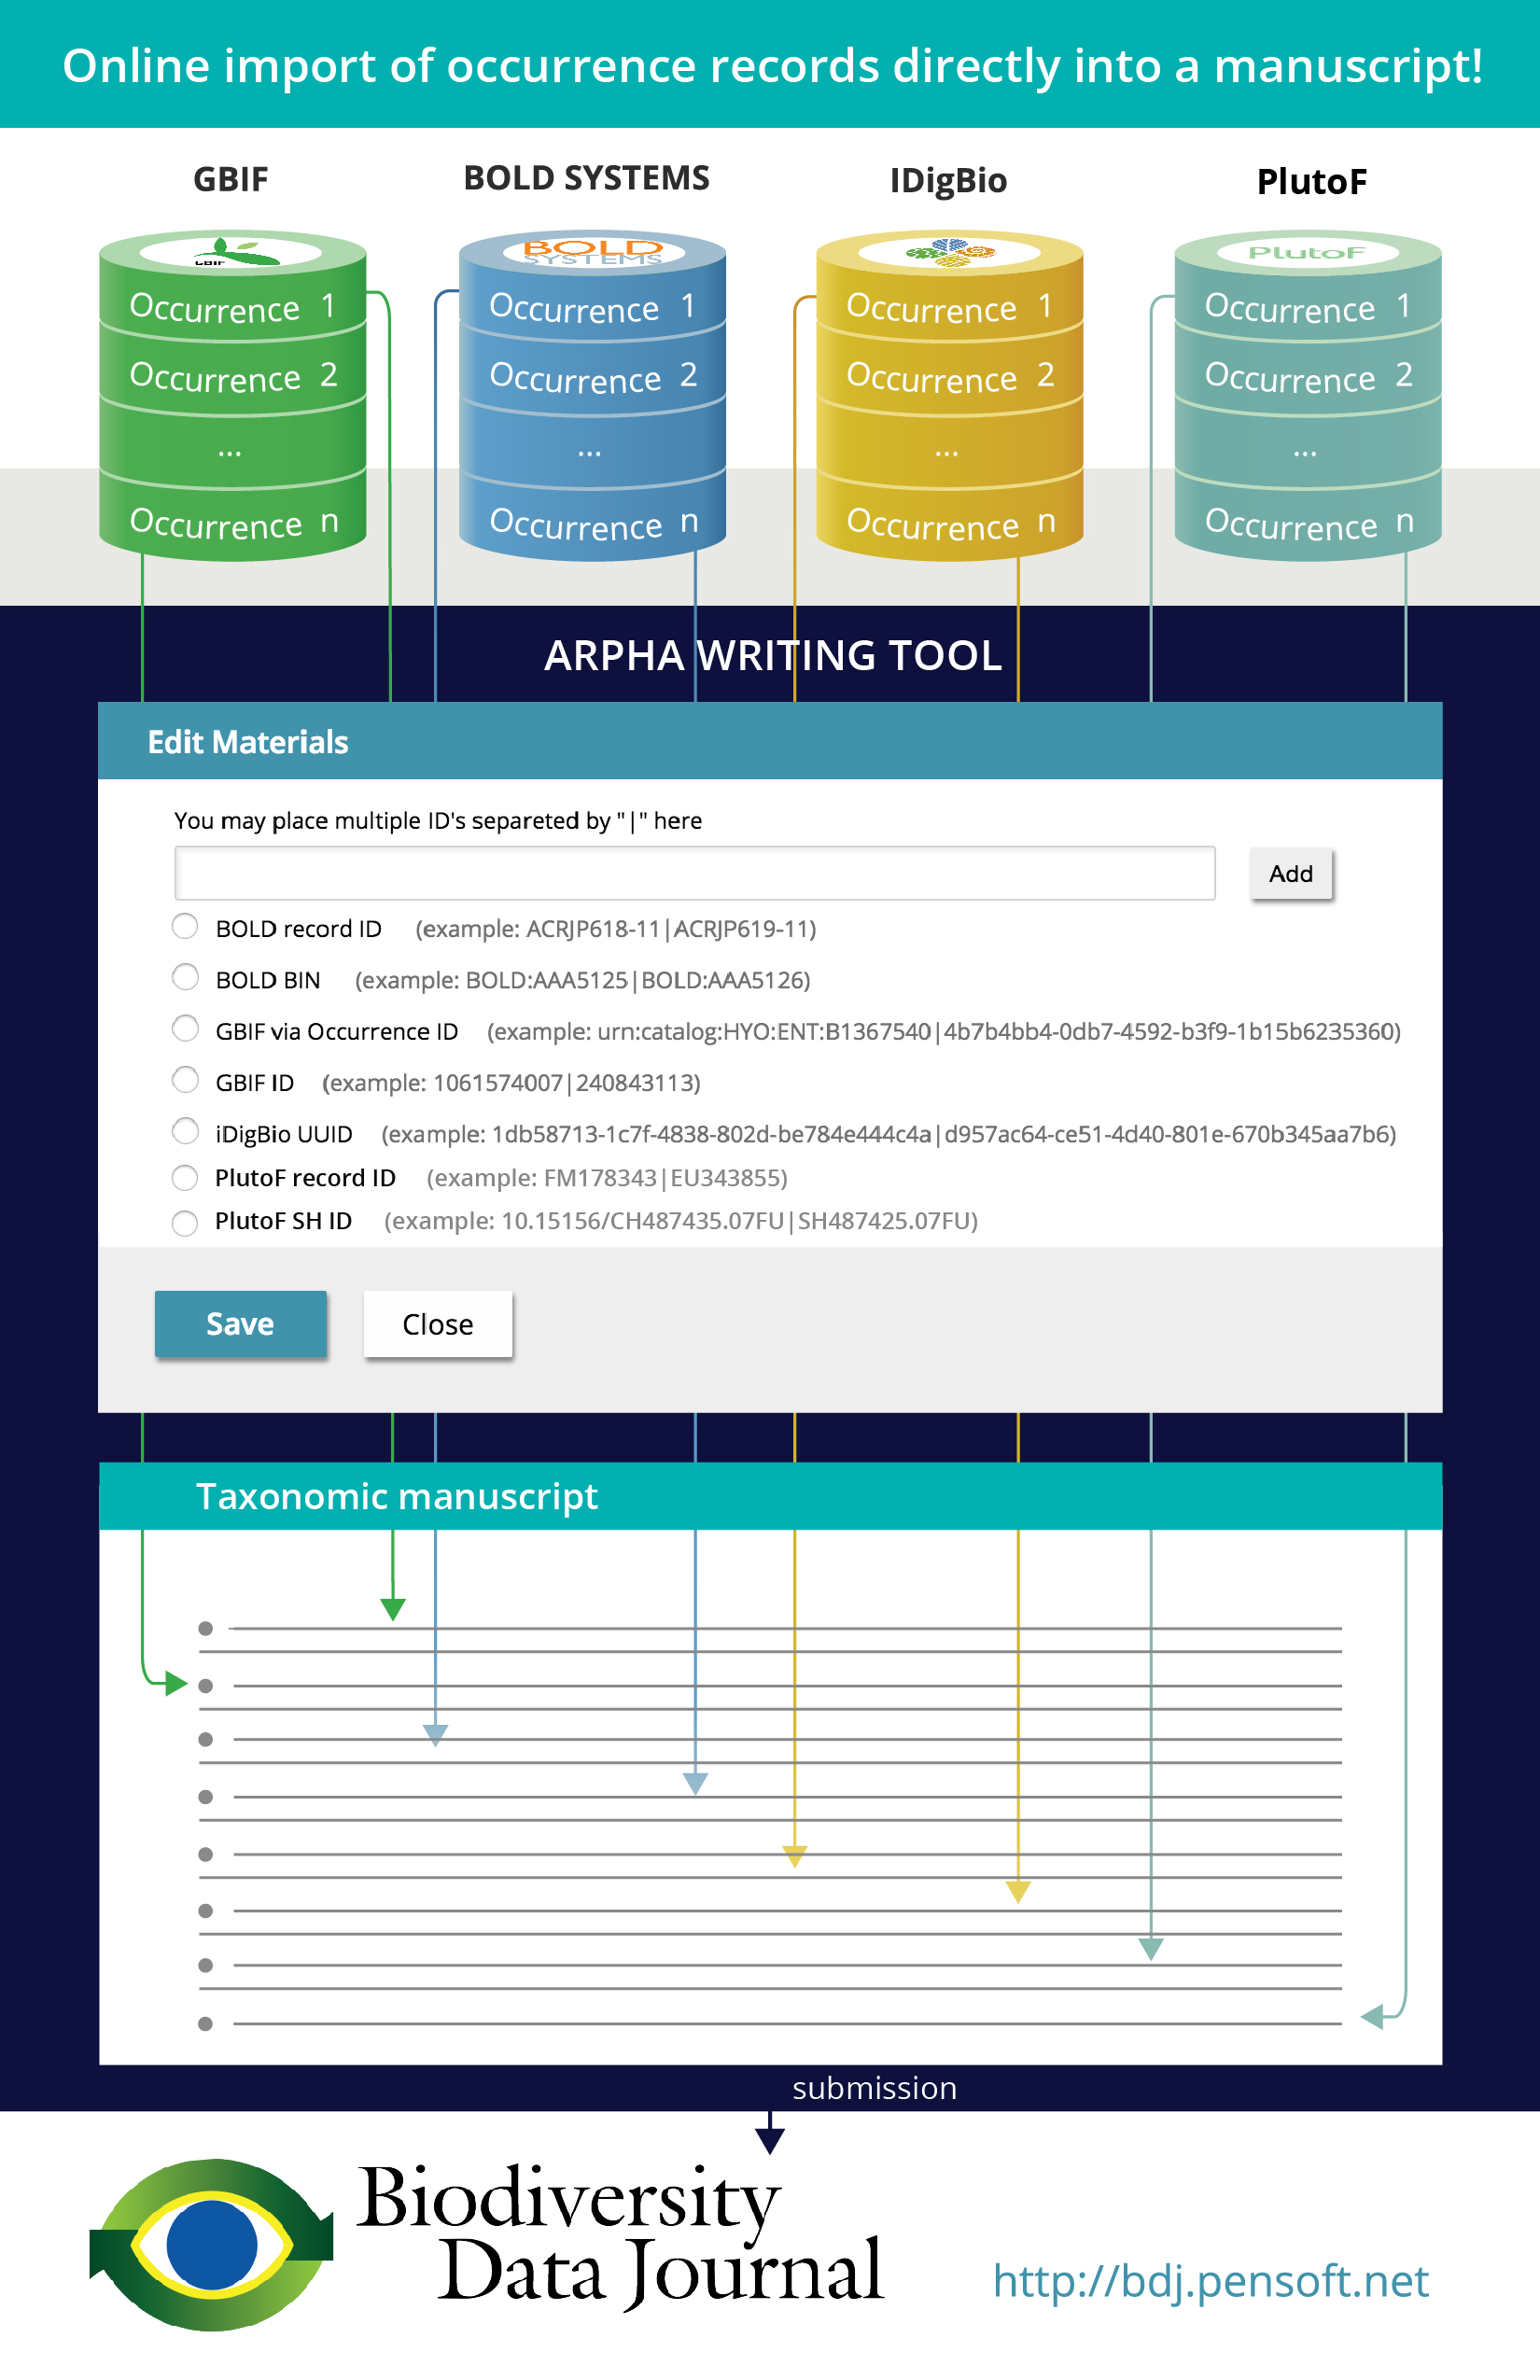
\includegraphics[width=\textwidth]{Figures/workflow-idigbio}
\decoRule
\caption{Работният поток от информационните портали GBIF, BOLD Systems, iDigBio и PlutoF чрез елементи на потребителски интерфейс в AWT.}
\label{fig:workflow-idigbio}
\end{figure}

\begin{figure}
\centering
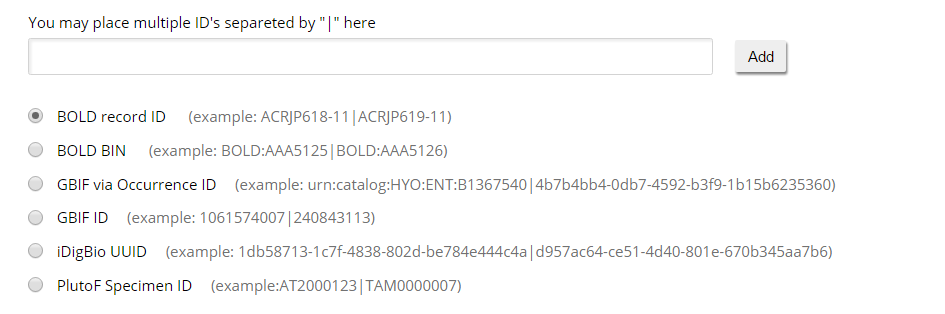
\includegraphics[width=\textwidth]{Figures/occurrence-input-mask}
\decoRule
\caption{Потребителски интерфейс на ARPHA Writing Tool, контролиращ импортирането на записи на образци от външни бази данни.}
\label{fig:occurrence-input-mask}
\end{figure}

\subsection {Workflow 2: Автоматизирано генериране на ръкопис от Ecological Metadata Lanaguage (EML) метаданни в ARPHA Writing Tool}

Създадохме работен процес, който позволява на авторите да създават автоматично ръкописни материали от метаданни, съхранявани в EML (фиг. -\ref{fig:EML-download}, фиг.~\ref{fig:user-interface}).
\begin{figure}
\centering
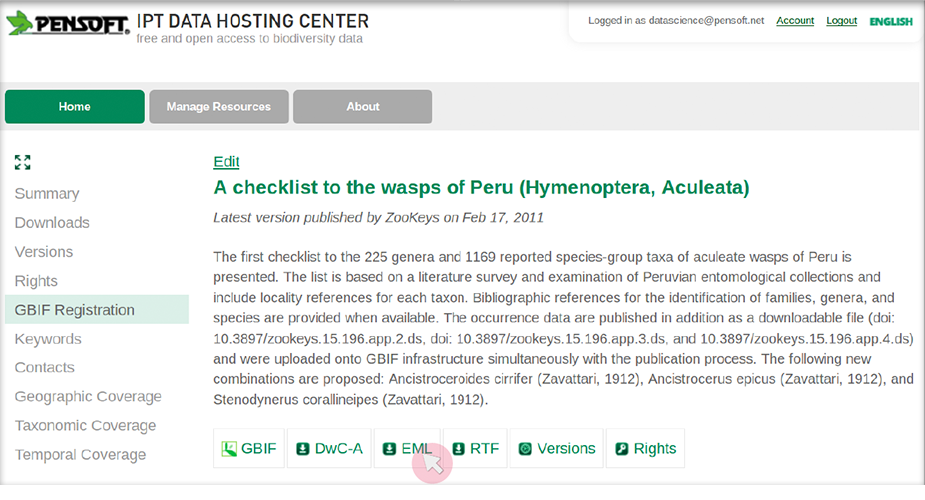
\includegraphics[width=\textwidth]{Figures/EML-download}
\decoRule
\caption{Изтегляне на EML от GBIF Integrated Publishing Toolkit (IPT).}
\label{fig:EML-download}
\end{figure}

\begin{figure}
\centering
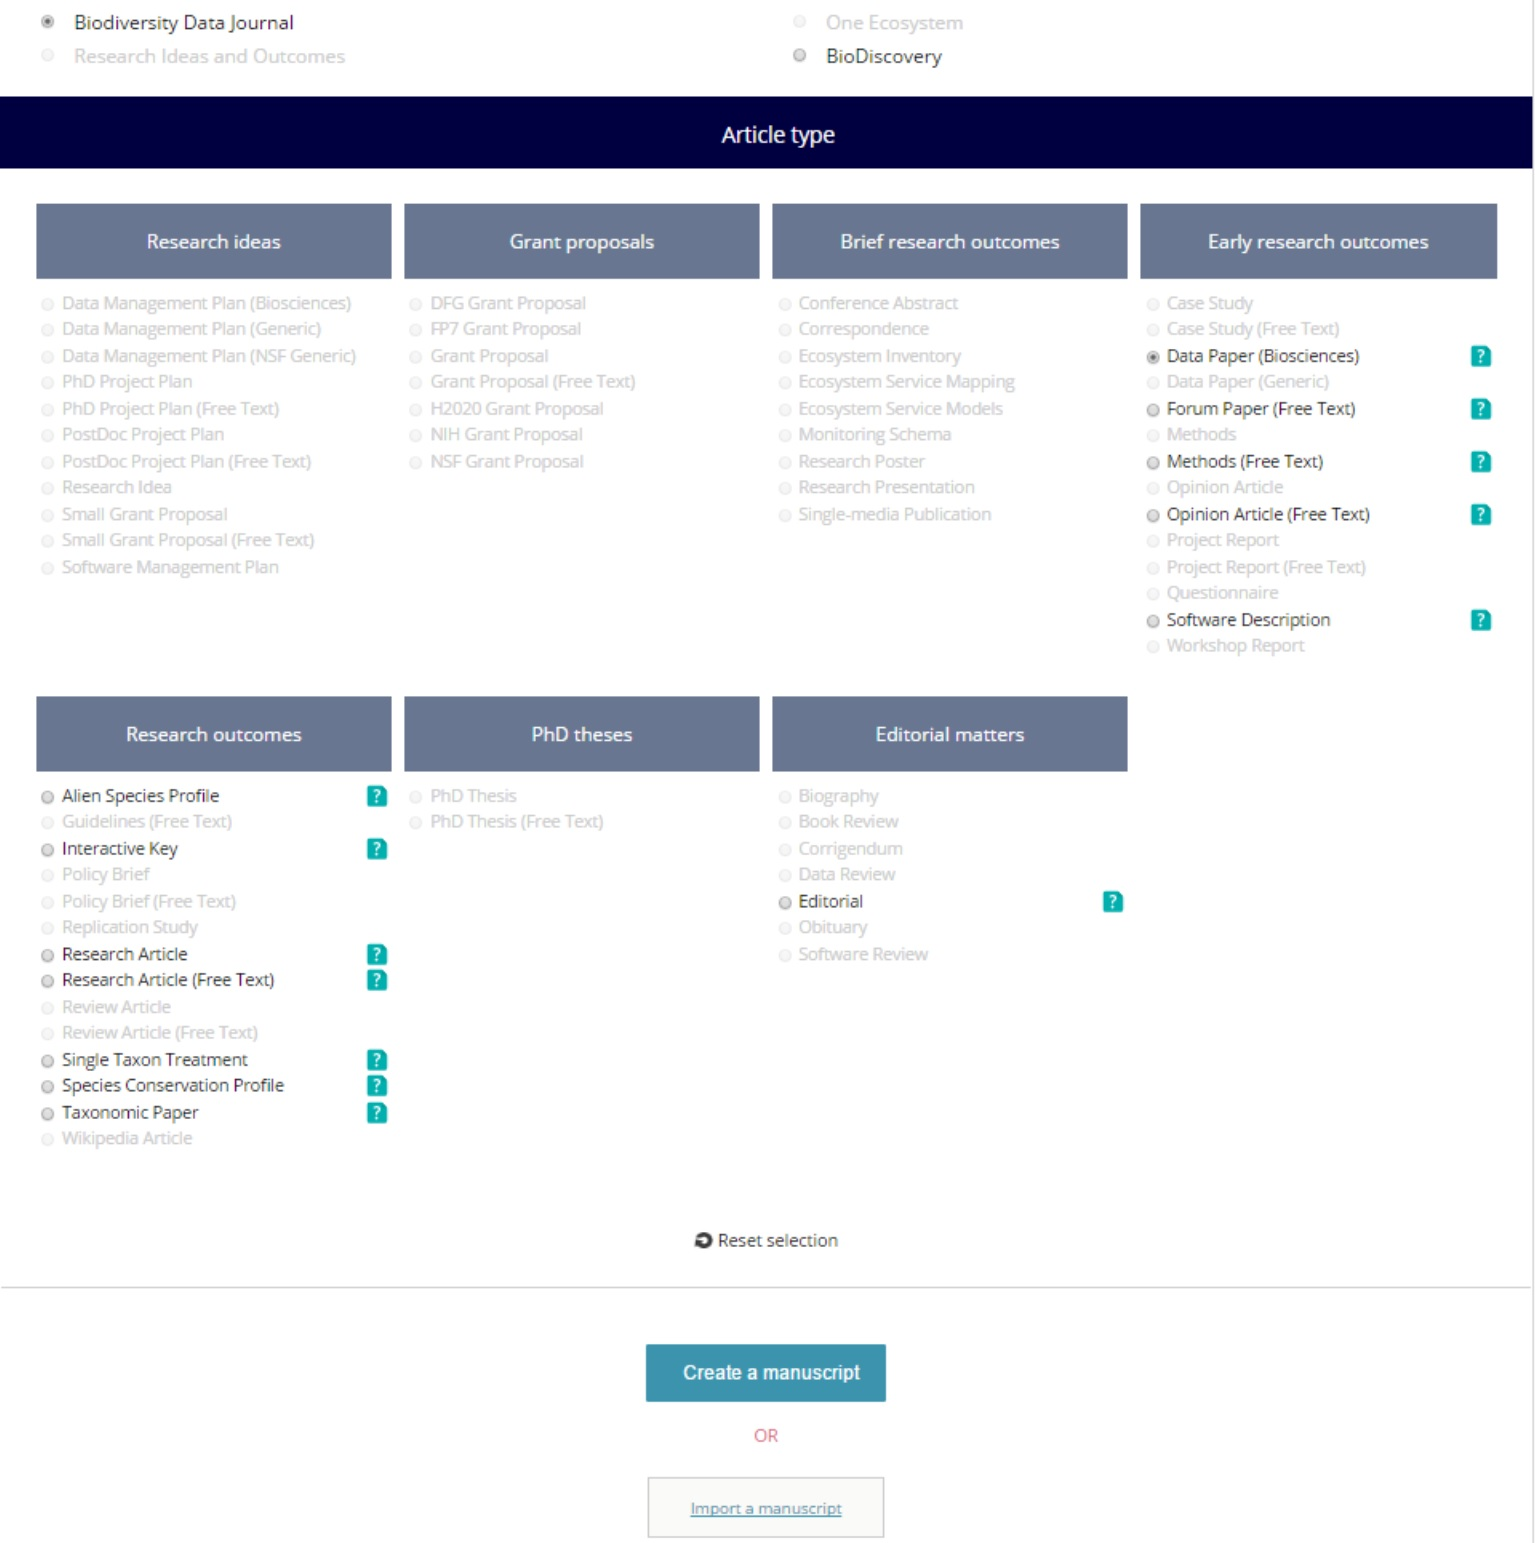
\includegraphics[width=\textwidth]{Figures/journal-selection}
\decoRule
\caption{Избор на списанието и шаблона "Data Paper (Biosciences)" в ARPHA Writing Tool.}
\label{fig:journal-selection}
\end{figure}

\begin{figure}
\centering
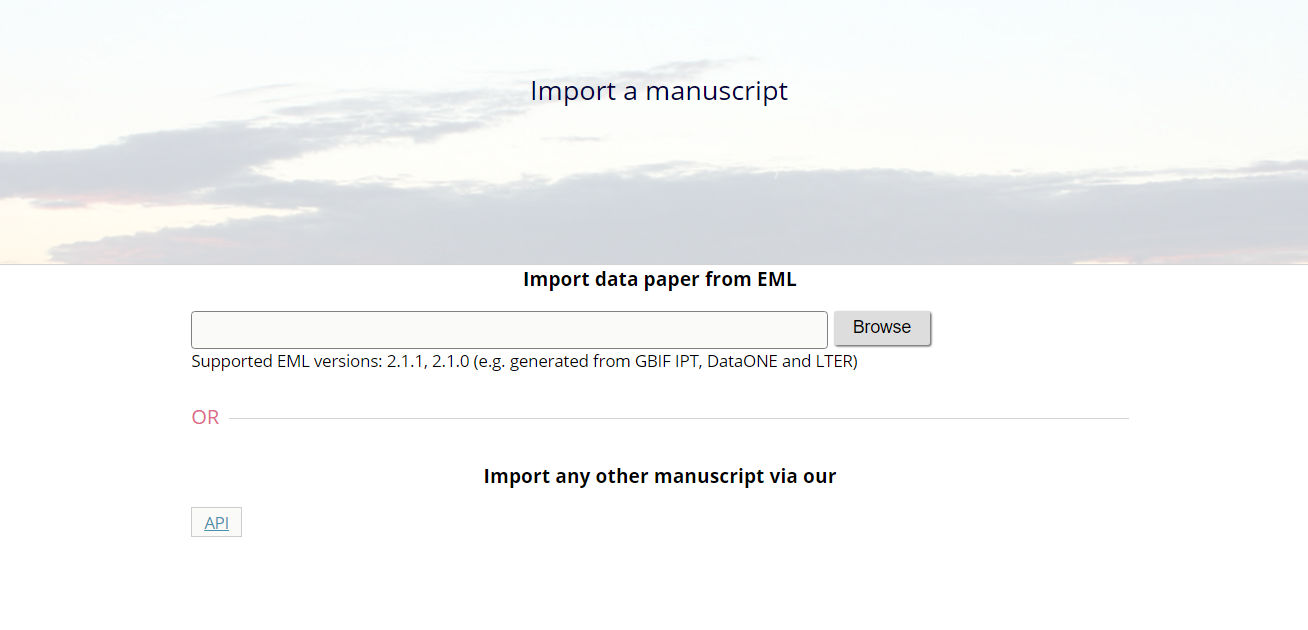
\includegraphics[width=\textwidth]{Figures/user-interface}
\decoRule
\caption{Полето за потребителски интерфейс за качване на EML файлове в ARPHA.}
\label{fig:user-interface}
\end{figure}